\documentclass{amsart}

\usepackage[T1]{fontenc}
\usepackage{enumerate, amsmath, amsfonts, amssymb, amsthm, mathrsfs, wasysym, graphics, graphicx, xcolor, url, hyperref, hypcap, shuffle, xargs, multicol, overpic, pdflscape, multirow, hvfloat, minibox, accents, array, multido, xifthen, a4wide, ae, aecompl, blkarray, pifont, mathtools, etoolbox, dsfont}
\usepackage{marginnote}
\hypersetup{colorlinks=true, citecolor=darkblue, linkcolor=darkblue}
\usepackage[all]{xy}
\usepackage[bottom]{footmisc}
\usepackage{tikz}
%\usepackage{tkz-graph}
%\usepackage{tikz-qtree}
\usetikzlibrary{trees, decorations, decorations.markings, shapes, arrows, matrix, calc, fit, intersections, patterns, angles, cd}
\usepackage[external]{forest}
%\tikzexternalize
\graphicspath{{figures/}{figures/nodes/}}
\makeatletter\def\input@path{{figures/}}\makeatother
\usepackage{caption}
\captionsetup{width=\textwidth}
\renewcommand{\topfraction}{1} % possibility to have one page of pictures
\renewcommand{\bottomfraction}{1} % possibility to have one page of pictures
\usepackage[noabbrev,capitalise]{cleveref}
\usepackage[export]{adjustbox}
\usepackage{ulem}\normalem

%%%%%%%%%%%%%%%%%%%%%%%%%%%%%%%%%%%%%%

% theorems
\newtheorem{theorem}{Theorem}%[section]
\newtheorem{corollary}[theorem]{Corollary}
\newtheorem{proposition}[theorem]{Proposition}
\newtheorem{lemma}[theorem]{Lemma}
\newtheorem{conjecture}[theorem]{Conjecture}
\newtheorem*{theorem*}{Theorem}%[section]

\theoremstyle{definition}
\newtheorem{definition}[theorem]{Definition}
\newtheorem{example}[theorem]{Example}
\newtheorem{remark}[theorem]{Remark}
\newtheorem{question}[theorem]{Question}
\newtheorem{problem}[theorem]{Problem}
\newtheorem{notation}[theorem]{Notation}
\newtheorem{assumption}[theorem]{Assumption}
\crefname{notation}{Notation}{Notations}
\crefname{problem}{Problem}{Problems}
 
% math special letters
\newcommand{\R}{\mathbb{R}} % reals
\newcommand{\N}{\mathbb{N}} % naturals
\newcommand{\Z}{\mathbb{Z}} % integers
\newcommand{\C}{\mathbb{C}} % complex
\newcommand{\I}{\mathbb{I}} % set of integers
\newcommand{\HH}{\mathbb{H}} % hyperplane
\newcommand{\K}{\mathbb{K}} % field
\newcommand{\fA}{\mathfrak{A}} % alternating group
\newcommand{\fB}{\mathfrak{S}^\textsc{b}} % signed symmetric group
\newcommand{\cA}{\mathcal{A}} % algebra
\newcommand{\cC}{\mathcal{C}} % collection
\newcommand{\cS}{\mathcal{S}} % ground set
\newcommand{\uR}{\underline{R}} % underline set
\newcommand{\uS}{\underline{S}} % underline set
\newcommand{\uT}{\underline{T}} % underline set
\newcommand{\oS}{\overline{S}} % overline set
\newcommand{\ucS}{\underline{\cS}} % underline ground set
\renewcommand{\c}[1]{\mathcal{#1}} % caligraphic letters
\renewcommand{\b}[1]{{\boldsymbol{#1}}} % bold letters
\newcommand{\bb}[1]{\mathbb{#1}} % bb letters
\newcommand{\f}[1]{\mathfrak{#1}} % frak letters
\newcommand{\h}{\widehat} % hat letters

% math commands
\newcommand{\set}[2]{\left\{ #1 \;\middle|\; #2 \right\}} % set notation
\newcommand{\bigset}[2]{\big\{ #1 \;\big|\; #2 \big\}} % big set notation
\newcommand{\Bigset}[2]{\Big\{ #1 \;\Big|\; #2 \Big\}} % Big set notation
\newcommand{\setangle}[2]{\left\langle #1 \;\middle|\; #2 \right\rangle} % set notation
\newcommand{\ssm}{\smallsetminus} % small set minus
\newcommand{\dotprod}[2]{\left\langle \, #1 \; \middle| \; #2 \, \right\rangle} % dot product
\newcommand{\symdif}{\,\triangle\,} % symmetric difference
\newcommand{\one}{\b{1}} % the all one vector
\newcommand{\eqdef}{\mbox{\,\raisebox{0.2ex}{\scriptsize\ensuremath{\mathrm:}}\ensuremath{=}\,}} % :=
\newcommand{\defeq}{\mbox{~\ensuremath{=}\raisebox{0.2ex}{\scriptsize\ensuremath{\mathrm:}} }} % =:
\newcommand{\simplex}{\b{\triangle}} % simplex
\renewcommand{\implies}{\Rightarrow} % imply sign
\newcommand{\transpose}[1]{{#1}^t} % transpose matrix

% operators
\DeclareMathOperator{\conv}{conv} % convex hull
\DeclareMathOperator{\vect}{vect} % linear span
\DeclareMathOperator{\cone}{cone} % cone hull
\DeclareMathOperator{\inv}{inv} % inversions
\DeclareMathOperator{\ninv}{ninv} % inversions
\DeclareMathOperator{\Ima}{Im} % image
\DeclareMathOperator{\Vol}{Vol} % (mixed) volume

% others
\newcommand{\ie}{\textit{i.e.}~} % id est
\newcommand{\eg}{\textit{e.g.}~} % exempli gratia
\newcommand{\Eg}{\textit{E.g.}~} % exempli gratia
\newcommand{\apriori}{\textit{a priori}} % a priori
\newcommand{\viceversa}{\textit{vice versa}} % vice versa
\newcommand{\versus}{\textit{vs.}~} % versus
\newcommand{\aka}{\textit{a.k.a.}~} % also known as
\newcommand{\perse}{\textit{per se}} % per se
\newcommand{\ordinal}{\textsuperscript{th}} % th for ordinals
\newcommand{\ordinalst}{\textsuperscript{st}} % st for ordinals
\definecolor{darkblue}{rgb}{0,0,0.7} % darkblue color
\definecolor{green}{RGB}{57,181,74} % darkblue color
\definecolor{violet}{RGB}{147,39,143} % darkblue color
\newcommand{\darkblue}{\color{darkblue}} % darkblue command
\newcommand{\defn}[1]{\textsl{\darkblue #1}} % emphasis of a definition
\newcommand{\para}[1]{\smallskip\noindent\uline{#1.}} % paragraph
\renewcommand{\topfraction}{1} % possibility to have one page of pictures
\renewcommand{\bottomfraction}{1} % possibility to have one page of pictures
%\renewcommand\labelitemi{$\diamond$} % redefine itemize default symbol

% marginal comments
\usepackage{todonotes}
\newcommand{\vincent}[1]{\todo[color=blue!30]{\rm #1 \\ \hfill --- V.}}
\newcommand{\Vincent}[1]{\todo[inline, color=blue!30]{\rm #1 \\ \hfill --- V.}}
\newcommand{\jean}[2][]{\todo[size=\scriptsize, color=orange!30,#1]{\rm #2 \\ \hfill --- J.}}
\newcommand{\Jean}[2][]{\todo[inline, size=\scriptsize, color=orange!30,#1]{\rm #2 \\ \hfill --- J.}}

% lattices
\newcommand{\meet}{\wedge} % meet
\newcommand{\join}{\vee} % join
\newcommand{\bigMeet}{\bigwedge} % meet
\newcommand{\bigJoin}{\bigvee} % join
\newcommandx{\projDown}[1][1={}]{\smash{\pi_\downarrow^{#1}}} % down projection map
\newcommandx{\projUp}[1][1={}]{\smash{\pi^\uparrow_{#1}}} % up projection map
\newcommand{\con}{\mathrm{con}} % congruence

% geometry
\newcommandx{\Fan}[1][1=D]{\mathcal{F}_{#1}} % fan
\newcommand{\polytope}[1]{\mathds{#1}} % font polytope

% specific rectangulotope
\newcommand{\Asso}{\polytope{A}\mathsf{sso}} % associahedron
\newcommand{\WRP}{\polytope{WRP}} % weak rectangulation polytope
\newcommand{\SRP}{\polytope{SRP}} % strong rectangulation polytope
\newcommand{\horizontalPattern}{\smash{\raisebox{-.15cm}{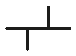
\includegraphics[scale=.5]{horizontalPattern}}}} % horizontal pattern
\newcommand{\verticalPattern}{\smash{\raisebox{-.25cm}{
\includegraphics[scale=.5]{verticalPattern}}}} % vertical pattern

% formating the table of contents
\setcounter{tocdepth}{4}
\makeatletter
\def\l@part{\@tocline{1}{8pt}{0pc}{}{}}
\def\l@section{\@tocline{1}{4pt}{0pc}{}{}}
\makeatother
\let\oldtocpart=\tocpart
\renewcommand{\tocpart}[2]{\sc\large\oldtocpart{#1}{#2}}
\let\oldtocsection=\tocsection
\renewcommand{\tocsection}[2]{\bf\oldtocsection{#1}{#2}}
\let\oldtocsubsubsection=\tocsubsubsection
\renewcommand{\tocsubsubsection}[2]{\quad\oldtocsubsubsection{#1}{#2}}

%%%%%%%%%%%%%%%%%%%%%%%%%%%%%%%%%%%%%%

\title{Rectangulation polytopes}

\thanks{VP was partially supported by the Spanish grant PID2022-137283NB-C21 of MCIN/AEI/10.13039/501100011033 / FEDER, UE, by Departament de Recerca i Universitats de la Generalitat de Catalunya (2021 SGR 00697), by the French grant CHARMS (ANR-19-CE40-0017), and by the French--Austrian projects PAGCAP (ANR-21-CE48-0020 \& FWF I 5788).}

\author{Jean Cardinal}
\address{Université Libre de Bruxelles}
\email{jean.cardinal@ulb.be}
\urladdr{\url{https://jean.cardinal.web.ulb.be}}

\author{Vincent Pilaud}
\address{Universitat de Barcelona}
\email{vincent.pilaud@ub.edu}
\urladdr{\url{https://www.ub.edu/comb/vincentpilaud/}}

%%%%%%%%%%%%%%%%%%%%%%%%%%%%%%%%%%%%%%

\begin{document}

\begin{abstract}
\end{abstract}

\maketitle

\tableofcontents

%%%%%%%%%%%%%%%%%%%%%%%%%%%%%%%%%%%%%%

\section{Introduction}

%%%%%%%%%%%%%%%%%%%%%%%%%%%%%%%%%%%%%%

\newpage
\section{Rectangulations}
\label{sec:rectangulations}

%%%%%%%%%%%%

\subsection{Combinatorics of (generic) rectangulations}
\label{subsec:rectangulations}

\Vincent{
Note that there seem to be a canonical integer drawing of~$R$ described as follows.
For vertical segment~$v$ of~$R$, consider the path~$p$ passing through~$v$ with maximal slope.
The abscissa of~$v$ is then the number of rectangle on the left of~$p$ plus the number of \horizontalPattern{} patterns along~$p$ before~$v$ minus the number of \horizontalPattern{} patterns along~$p$ after~$v$.
The ordinate of an horizontal segment~$h$ of~$R$ is defined symmetrically.
}

%%%%%%%%%%%%

\subsection{Source and target trees of a rectangulation}
\label{subsec:sourceTargetTrees}

\begin{figure}
	\centerline{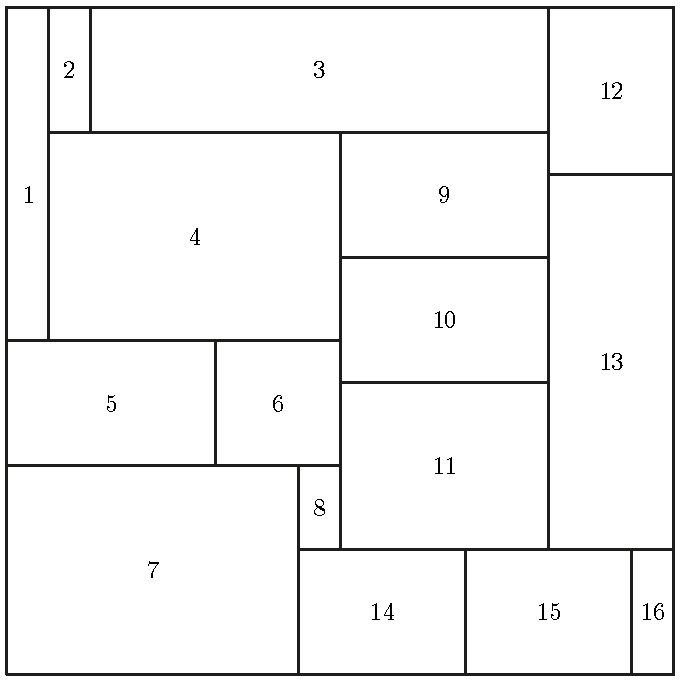
\includegraphics[scale=.7]{strongRectangulation} \qquad 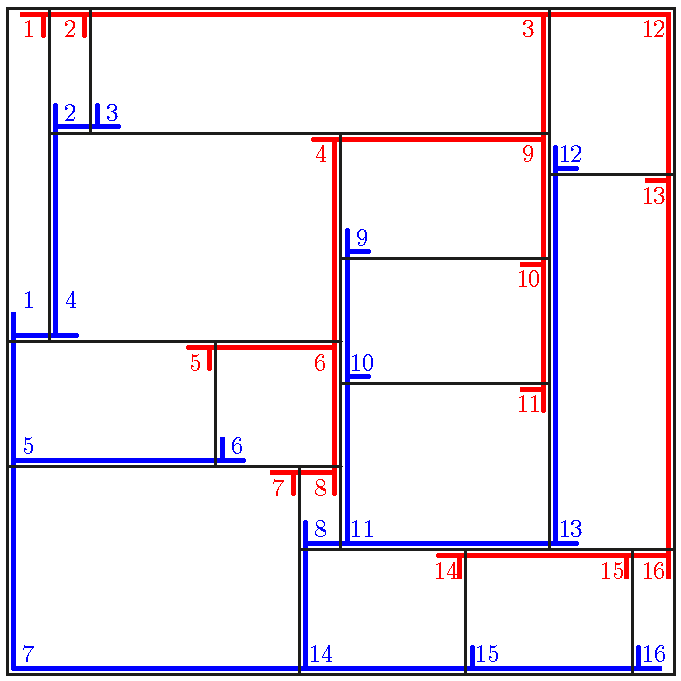
\includegraphics[scale=.7]{strongRectangulationTrees}}
	\caption{A strong rectangulation (left) and its pair of intertwining twin trees (right). The corresponding $2$-clumped permutation is $[7,5,14,8,1,6,15,11,4,10,16,2,9,13,3,12]$ and its inverse is $[5, 12, 15, 9, 2, 6, 1, 4, 13, 10, 8, 16, 14, 3, 7, 11]$. Example from \cite{AsinowskiCardinalFelsnerFusy}.}
\end{figure}

Fix a rectangulation~$R$ with $n$ rectangles, and consider the directed graph~$D(R)$ whose vertex set is the set of all vertices of~$R$, and whose edges are obtained as follows.
For each rectangle~$r$ of~$R$, we include in~$D(R)$ four edges joining the vertices of~$r$, where the horizontal edges are oriented from left to right if they are horizontal, and the vertical edges are oriented from bottom to top if they are vertical.
Hence, the bottom left corner of~$r$ is its source~$s(r)$, while its top right corner is its target~$t(r)$.
Note that since~$R$ is generic, the sources~$\set{s(r)}{r \in [n]}$ and the targets~$\set{t(r)}{r \in [n]}$ are disjoint.
The \defn{source tree}~$S(R)$ (resp.~\defn{target tree}~$T(R)$) is the subgraph of~$D(R)$ induced by the sources~$\set{s(r)}{r \in [n]}$ (resp.~by the targets~$\set{t(r)}{r \in [n]}$).
See \cref{fig:sourceTargetTrees}.

\begin{lemma}
The source tree~$S(R)$ (resp.~target tree~$T(R)$) is a binary tree, rooted at the bottom left (resp.~top right) corner of~$R$, and oriented from (resp.~towards) its root.
\end{lemma}

\begin{proof}
By symmetry, we only prove the statement for the source tree~$S(R)$.
As the triangulation is generic, each source~$s(r)$ distinct from the bottom left corner of~$R$ is either on the top edge of a rectangle~$r'$ or on the right edge of a rectangle~$r'$ (but not both).
This shows that~$r$ distinct from the bottom left rectangle of~$R$ has a unique parent~$r'$ in~$S(R)$, so that~$S(R)$ is indeed a tree on~$[n]$.
This tree is binary as each node has at most one vertical child and one horizontal child, and no other children.
\end{proof}

We complete each node of~$S(R)$ and~$T(R)$ with a vertical (resp.~horizontal) leaf if it has no vertical (resp.~horizontal) child.
See \cref{fig:sourceTargetTrees}.
Recall that the \defn{inorder labeling} of a binary tree~$T$ is the labeling of the nodes of~$T$ such that the label of each node~$t$ of~$T$ is larger than all labels in the left subtree of~$t$ and larger than all labels in the right subtree of~$t$.

\begin{lemma}
For any rectangle~$r$ of~$R$, the inorder label of the source~$s(r)$ in~$S(R)$ coincides with the inorder label of the target~$t(r)$ in~$T(R)$.
\end{lemma}

\begin{proof}
\end{proof}

This enables to unambiguously label the rectangles of~$R$ by the inorder 
The resulting labeling coincides with the NW--SE labeling of~\cite{AsinowskiCardinalFelsnerFusy}.
We prefer our presentation with~$S(R)$ and~$T(R)$ here as we will actually use these two binary trees.

\begin{lemma}
The source tree~$S(R)$ and target tree~$T(R)$ are \defn{twin binary trees}, meaning that they satisfy the following equivalent conditions:
\begin{enumerate}[(i)]
\item $S$ and~$T$ admit a common linear extension,
\item for any~$i \in [n-1]$, the node~$i$ is in the left subtree of the node~$i+1$ in~$S$ if and only if the node~$i+1$ is in the right subtree of the node~$i$ in~$R$,
\item for any~$i \in [n-1]$, the $(i+1)$-st leaf of~$S$ is a left leaf if and only if the $(i+1)$-st leaf of~$R$ is a right leaf.
\end{enumerate}
\end{lemma}

\begin{proof}
\end{proof}

%%%%%%%%%%%%

\subsection{Rectangulation insertion of permutations}
\label{subsec:insertion}

\Vincent{If my canonical drawing indeed makes sense, I would love to describe the insertion map directly on rectangles.}

\Vincent{Describe the strong poset here?}

The insertion fiber of a rectangulation~$R$ precisely consists in the linear extensions of the strong poset.

%%%%%%%%%%%%

\subsection{Diagonal rectangulations}
\label{subsec:diagonalRectangulations}

\begin{figure}
	\centerline{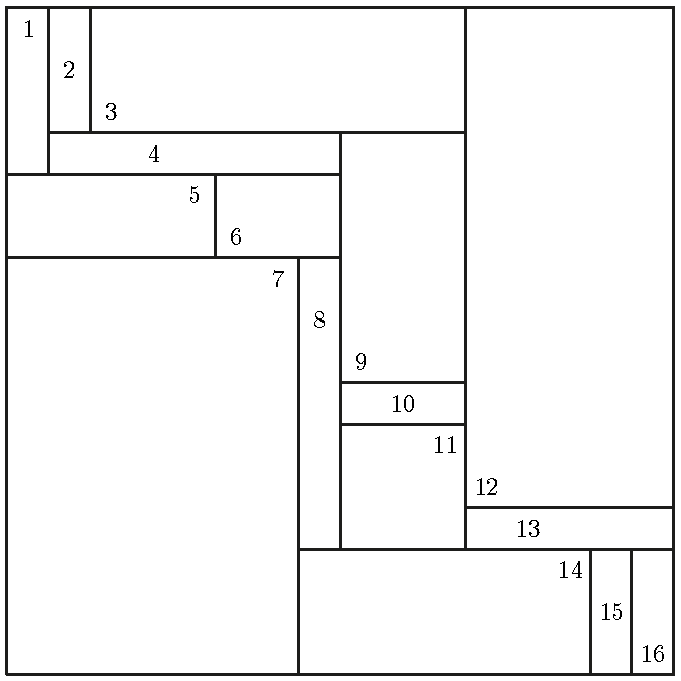
\includegraphics[scale=.7]{weakRectangulation} \qquad 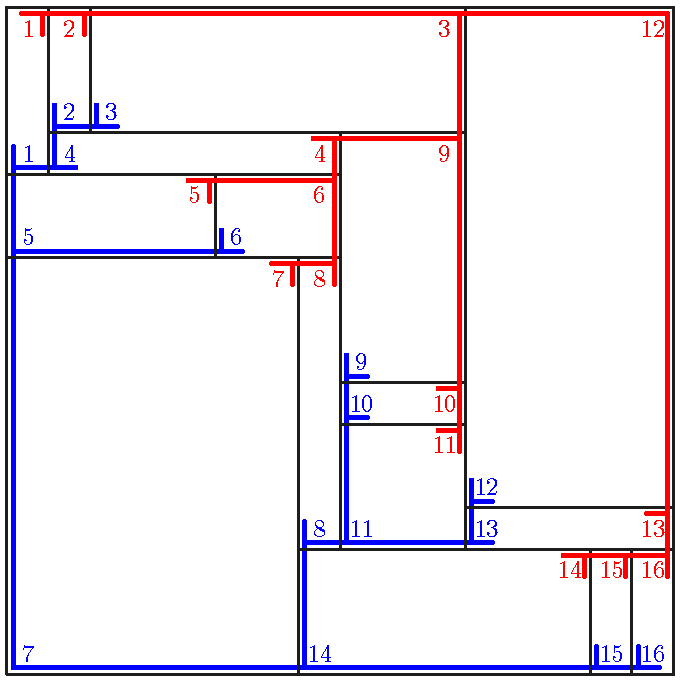
\includegraphics[scale=.7]{weakRectangulationTrees}}
	\caption{A weak rectangulation (left) and its pair of separated twin trees (right). The corresponding cotwisted Baxter permutation is $[7,14,15,16,8,11,13,10,5,6,1,4,9,2,3,12]$ and its inverse is $[11, 14, 15, 12, 9, 10, 1, 5, 13, 8, 6, 16, 7, 2, 3, 4]$.}
\end{figure}

We call \defn{antidiagonal} the segment joining the top left corner to the bottom right corner.
A rectangulation~$R$ is \defn{diagonal} (or \defn{weak}) if it satisfies the following equivalent conditions:
\begin{enumerate}[(i)]
\item all rectangles of~$R$ meet the antidiagonal,
\item the source~$s(r)$ (resp.~target~$t(r)$) of each rectangle~$r$ of~$R$ is below (resp.~above) the antidiagonal,
\item the source tree~$S(R)$ (resp.~target tree~$T(R)$) remains below (resp.~above) the antidiagonal,
\item the source tree~$S(R)$ and the target tree~$T(R)$ do not overlap along a segment of~$R$,
\item $R$ avoids the patterns \horizontalPattern{} and \verticalPattern{},
\item the $2$-clumped permutation~$\projDown(R)$ avoids the patterns~$2413$ and~$3412$,
\item the co-$2$-clumped permutation~$\projDown(R)$ avoids the patterns~$2143$ and~$3142$,
\end{enumerate}

%%%%%%%%%%%%%%%%%%%%%%%%%%%%%%%%%%%%%%

\section{Quotientopes}
\label{sec:quotientopes}

%%%%%%%%%%%%%%%%%%%%%%%%%%%%%%%%%%%%%%

\section{Weak rectangulation polytope}
\label{sec:weakRectangulationPolytope}

%%%%%%%%%%%%%%%%%%%%%%%%%%%%%%%%%%%%%%

\section{Strong rectangulation polytope}
\label{sec:weakRectangulationPolytope}

%%%%%%%%%%%%%%%%%%%%%%%%%%%%%%%%%%%%%%

%\clearpage
\addtocontents{toc}{ \vspace{.1cm} }
\bibliographystyle{alpha}
\bibliography{rectangulotopes}
\label{sec:biblio}

\end{document}
